\documentclass[12pt,a4paper]{article}
\usepackage[utf8]{inputenc}
\usepackage[danish]{babel}
\usepackage{amsmath}
\usepackage{amsfonts}
\usepackage{amssymb}
\usepackage{graphicx}
\usepackage[left=2cm,right=2cm,top=2cm,bottom=2cm]{geometry}

%KEMI ORBITAL SRP%

\usepackage[x11names]{xcolor}
\usepackage{tcolorbox}% no need in this mwe
\usepackage[font=small]{caption}% no need in this mwe
\usepackage{float}% no need in this mwe
\usepackage{floatflt}% no need in this mwe

\usepackage{tikz} 
\usepackage{tikzorbital}
\usetikzlibrary{fadings,patterns,backgrounds,fit,arrows}
\pgfdeclarelayer{backbackground}
\pgfsetlayers{backbackground,background,main}

%%%%%%%%%%%%%%%%%%%%%%%%%%%%%%%%%%%%%%%%

\usepackage{titlepic}
\usepackage{enumerate}
\usepackage{enumitem}
\usepackage{float}
\usepackage{pdfpages}
\usepackage[colorlinks = true,
            linkcolor = blue,
            urlcolor  = blue,
            citecolor = blue,
            anchorcolor = blue]{hyperref}
\usepackage[explicit]{titlesec}
\usepackage{pstricks}
\usepackage[amsmath,thmmarks]{ntheorem} %pakke til at lave sætningsenvorinmets (kan ikke loades sammen med amsthm)
\usepackage{color}
\usepackage{tikz}

%opretter environmets til sætningsstrukturen 
\theorembodyfont{\normalfont}

	
	%sætnings environment	
	\newtheorem{thm}{Sætning}

	\theoremstyle{break}	
	%opgave environment	
	\newtheorem{opg}{Opgave}	

	%Korrolar environment
	\newtheorem{korollar}[thm]{Korollar}	
	
	%Lemma environment	
	\newtheorem{lemma}[thm]{Lemma}
	
	\theoremsymbol{\ensuremath{\circ}}	
	
	%definition environment	
	\newtheorem{definition}[thm]{Definition}
	
	%eksempel environment	
	\newtheorem{eksempel}[thm]{Eksempel}
	
	
	
	%Bevis environment
	\theoremstyle{nonumberplain}
	\theoremheaderfont{%
	\normalfont\itshape}
	\theorembodyfont{\normalfont}
	\theoremsymbol{\ensuremath{\square}}
	\theoremseparator{.}
	
	\newtheorem{proof}{Bevis}
	\newtheorem{los}{Løsning}
	






\setlength\parindent{0pt}

%\titleformat{\section}{\Large\bfseries}{}{0pt}{#1}
%\titleformat{\subsection}{\large\bfseries}{}{0pt}{#1}


%nye komandoer
\newcommand{\mR}{\mathbb{R}}
\newcommand{\mZ}{\mathbb{Z}}
\newcommand{\mN}{\mathbb{N}}
\newcommand{\mQ}{\mathbb{Q}}
\newcommand{\mC}{\mathbb{C}}
\newcommand{\hs}{\hspace{2mm}}
\newcommand{\Hs}{\hspace{4mm}}
\newcommand{\pipe}{\hs | \hs}
\newcommand{\lp}{\left(}
\newcommand{\rp}{\right)}
\newcommand{\vect}[1]{\underline{#1}}
\newcommand{\matr}[1]{\underline{\underline{#1}}}
\newcommand{\cnum}[1]{\raisebox{.5pt}{\textcircled{\raisebox{-.9pt} {#1}}}}




\author{Sebastian Borgund Hansen \\ 3r, Nørre Gymnasium}
\title{SRP - Kemi \& Fysik}
\date{\today}



\begin{document}
\maketitle
\section{Kovalente bindinger i organiske molekyler}

Under visse omstændigheder vil to atomer der mødes danne et molekyle, hvor de to atomer er bundet sammen af en kovalent binding. I dette afsnit skal vi undersøge hvilke betingelser der netop gælder om denne type bindinger, der er grundlæggende for forståelsen af hvordan IR-spektra forekommer.

\subsection{Orbitaler}
For at forstå hvorfor to atomer vælger at gå sammen om at danne en binding hvori de deler deres elektroner er vi nødsaget til lige at betragte et enkelt atoms elektronkonfiguration. De subatomare entiteter som elektroner er opfører sig ikke lige så pænt som Bohr formulerede i hans atommodel, hvor elektronerne bevæger sig i cirkulære baner, eller skaller, rundt omkring atomets kerne. Ifølge nyere MOT (Læs: Molekylær Orbital Teori) har elektronerne en chance for at eksistere i visse områder omkring atomet. Disse områder er bestemt af hvor mange elektroner atomet har. Idéen om skallerne er ikke fuldstændig, men den molekylære orbital teori udbyggger de enkelte skaller, der behandles i Bohr model, med nogle undergrupper, som kaldes orbitaler. Det laveste energiniveau en elektron kan befinde sig i, når det bevæger sig rundt om atomkernen er kugleformet og har tildelt navnet 1s orbitalen. Figur 1 er en skitse af 1s orbitalen. 

\begin{figure}[ht!]
  \centering
  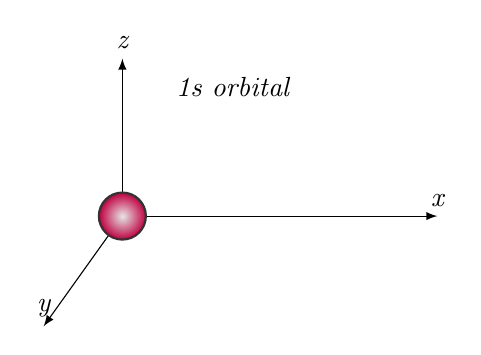
\begin{tikzpicture}[scale=2]
  \begin{scope}[font=\itshape]% to not type it every time, but better go for math mode


  \draw[-latex] (5,0)--(7,0) node[above]{x};
  \draw[-latex] (5,0)--(4.5,-0.7) node[above]{y};
  \draw[-latex] (5,0)--(5,1) node[above]{z};
  \orbital[color = purple, pos = {(5,0)}]{s} 
  \node[above] at (5.7,0.7) {1s orbital};

 		
  \end{scope}

  % correctly setting the background layer
  \begin{pgfonlayer}{backbackground}
  \fill[white](current bounding box.south west)rectangle
  (current bounding box.north east);
  \end{pgfonlayer}
  \end{tikzpicture}
  \caption{1s orbital} \end{figure}
  
  I s-orbitalerne er der plads til netop 2 elektroner. At den første orbital hedder 1s henviser til at den tilhører skal 1. I 2. skal tilhører elektronerne 2s orbitalen. s fordi at orbitalen er kugleformet og 2 fordi orbitalen knytter sig til 2. skal. Orbitalen ligner 1s orbitalen til forveksling, men vil have en større radius da elektronerne der befinder sig i denne orbital har mere energi. Da vi ved, at der skal være 8 elektroner i den 2. skal for, at oktetreglen er opfyldt og atomerne derfor er stabile mangler vi stadigvæk at placere 6 elektroner. Disse elektroner vil befinde sig i de såkaldte p-orbitaler. Der eksisterer 3 forskellige p-orbitaler, som ligner sløjfer og som hver især indeholder 2 elektroner. De tre p-orbitaler benævnes respektivt $p_x$, $p_y$ og $p_z$, da de er ortogonale på hinanden og ligger langs hhv. x, y og z aksen. De er på figur 2 illustreret i et kartesisk koordinatsystem.
  
TEST
 
\begin{figure}[ht!]
  \centering
  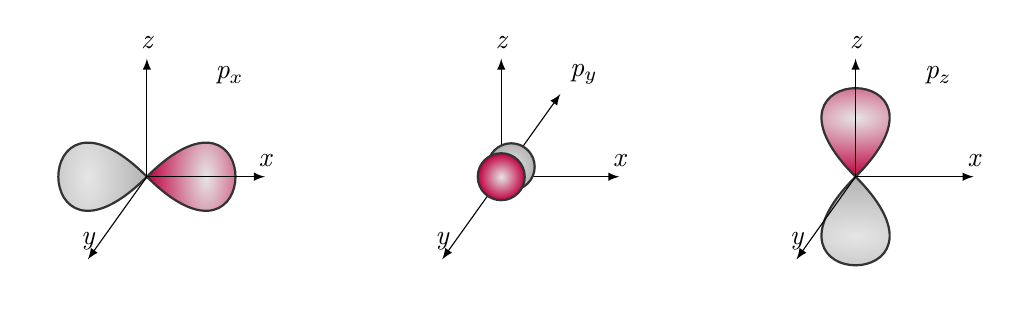
\begin{tikzpicture}[scale=1.5]
  \begin{scope}[font=\itshape]% to not type it every time, but better go for math mode

 \draw[-latex] (0,0)--(1,0) node[above]{x};
  \draw[-latex] (0,0)--(-0.5,-0.7) node[above]{y};
  \draw[-latex] (0,0)--(0,1) node[above]{z};
  \orbital[pcolor = purple, pos = {(0,0)}]{py}
  \node[above] at (0.7,0.7) {p$_x$};
	
  \draw[-latex] (3,0)--(3.5,0.7);
  \draw[-latex] (3,0)--(4,0) node[above]{x};
  \draw[-latex] (3,0)--(2.5,-0.7) node[above]{y};
  \draw[-latex] (3,0)--(3,1) node[above]{z};
  \orbital[pcolor = purple, pos = {(3,0)}]{px} 
  \node[above] at (3.7,0.7) {p$_y$};

  \draw[-latex] (6,0)--(7,0) node[above]{x};
  \draw[-latex] (6,0)--(5.5,-0.7) node[above]{y};
  \draw[-latex] (6,0)--(6,1) node[above]{z};
  \orbital[pcolor = purple, pos = {(6,0)}]{pz}
  \node[above] at (6.7,0.7) {p$_z$};
  \end{scope}
  % correctly setting the background layer
  \begin{pgfonlayer}{backbackground}
  \fill[white](current bounding box.south west)rectangle
  (current bounding box.north east);
  \end{pgfonlayer}
  \end{tikzpicture}
  \caption{$2p_x$, $2p_y$, $2p_z$ orbital} \end{figure}

I 3 skal kan der være 18 elektroner. Disse elektroner bliver først fyldt ind i en 3s orbital, der ligner både 1s og 2s orbitalen i og med, at den er kugleformet. Radius på 3s orbitalen er større end på 2s orbitalen grundet det højere energiniveau. 6 af de resterende 16 elektroner kan dernæst findes i 3p orbitalerne. Der er, ligesom 2p-orbitalerne, også tre 3p-orbitaler - $3p_x$,$3p_y$ og en $3p_z$ orbital. For det illustrative formål kan vi bare betragte 2p-orbitalerne. 3p-orbitalerne ligner dem, men elektronerne kan bare befinde sig i større sløjfer end 2p-orbitalerne. 

Nu har vi kigget på de simpleste af orbitalerne, s- og p-orbitalerne. Der eksisterer også d og f orbitaler. f-orbitalerne vil jeg ikke beskæftige mig med, men p-orbitalerne er illustretet  figur 3. (Se figur 3 og 4) 
\\

\begin{figure}[ht!]
  \centering
  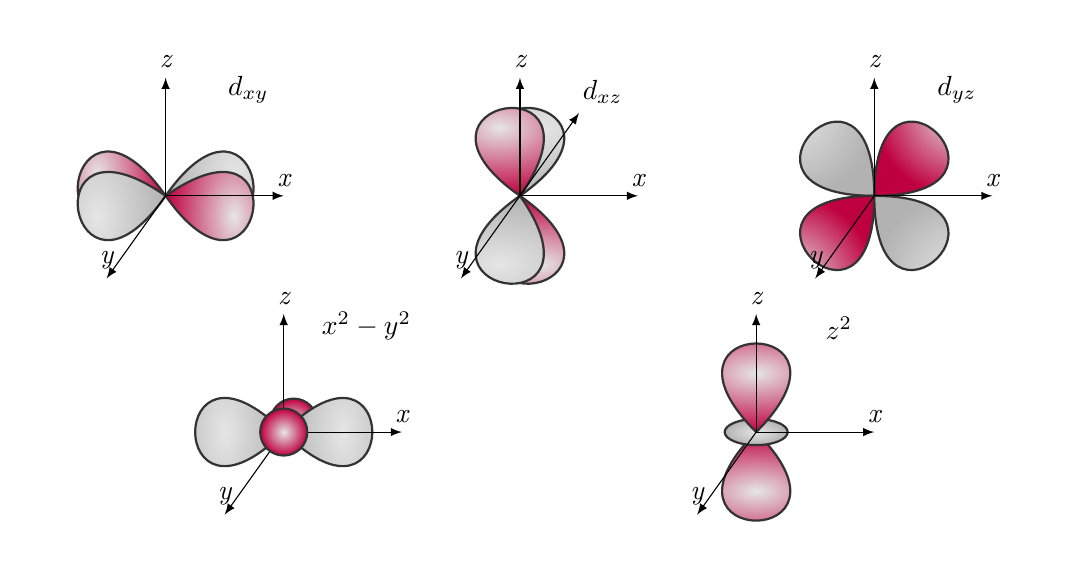
\begin{tikzpicture}[scale=1.5]
  \begin{scope}[font=\itshape]% to not type it every time, but better go for math mode

 \draw[-latex] (0,0)--(1,0) node[above]{x};
  \draw[-latex] (0,0)--(-0.5,-0.7) node[above]{y};
  \draw[-latex] (0,0)--(0,1) node[above]{z};
  \orbital[pcolor = purple, pos = {(0,0)}]{dxy}
  \node[above] at (0.7,0.7) {$d_{xy}$};
	
  \draw[-latex] (3,0)--(3.5,0.7);
  \draw[-latex] (3,0)--(4,0) node[above]{x};
  \draw[-latex] (3,0)--(2.5,-0.7) node[above]{y};
  \draw[-latex] (3,0)--(3,1) node[above]{z};
  \orbital[pcolor = purple, pos = {(3,0)}]{dxz} 
  \node[above] at (3.7,0.7) {$d_{xz}$};

  \draw[-latex] (6,0)--(7,0) node[above]{x};
  \draw[-latex] (6,0)--(5.5,-0.7) node[above]{y};
  \draw[-latex] (6,0)--(6,1) node[above]{z};
  \orbital[pcolor = purple, pos = {(6,0)}]{dyz}
  \node[above] at (6.7,0.7) {$d_{yz}$};
  
  \draw[-latex] (1,-2)--(2,-2) node[above]{x};
  \draw[-latex] (1,-2)--(0.5,-2.7) node[above]{y};
  \draw[-latex] (1,-2)--(1,-1) node[above]{z};
  \orbital[pcolor = purple, pos = {(1,-2)}]{dx2y2}
  \node[above] at (1.7,-1.3) {$x^{2}-y^{2}$};

  \draw[-latex] (5,-2)--(6,-2) node[above]{x};
  \draw[-latex] (5,-2)--(4.5,-2.7) node[above]{y};
  \draw[-latex] (5,-2)--(5,-1) node[above]{z};
  \orbital[pcolor = purple, pos = {(5,-2)}]{dz2}
  \node[above] at (5.7,-1.3) {$z^2$};
  
  \end{scope}
  % correctly setting the background layer
  \begin{pgfonlayer}{backbackground}
  \fill[white](current bounding box.south west)rectangle
  (current bounding box.north east);
  \end{pgfonlayer}
  \end{tikzpicture}
  \caption{$d_{xy}$, $d_{xz}$, $d_{yz}$, $x^{2}-y^{2}$, $z^2$ orbitalerne} 
  \end{figure}

\subsection{MO-teori}
I molekylær orbital teori, forkortet MO-teori, ses der på fordelingen af elektroner i molekyler på samme måde som vi ser på molekyler i atomer (FODNOTE TIL GENERAL CHEMISTRY s.149 mangler). Måden hvorpå vi bestemmer hvordan en elektron opfører sig på i et molekyle er ved hjælp af kvantemekanik og en bølgefunktion $\Psi$. På denne måde kan energien af en elektron og formen på det område hvori en elektron bevæger sig i bestemmes. Dette vil jeg kun berøre sporadisk. Som vi i afsnit 1.1 fandt ud af at elektroner i forskellige energiniveauer havde størst chance for at eksistere i forskellige områder som vi kaldte orbitaler, ligeså har elektroner i molekyler også orbitaler som de har en stor chance for at eksistere i. Forskellen er bare, at i molekyler kan elektronerne findes nær kernen på en hvilken som helst kerne, der indgår i molekylet; hvilket er hvorfor vi kalder disse orbitaler for molekylære elektronorbitaler eller bare molekylære orbitaler. 
Ligesom atomare orbitaler er molekyære orbitaler også fyldt når de indeholder præcist 2 orbitaler med modsat spin. 
\\

\subsubsection{$\pi$- \& $\sigma$-orbitaler}

Da vi så de atomare orbitaler gav vi dem navnene, s,p,d og f. Molekylære orbitaler har også navne, men jeg vil i denne opgave primært have fokus på hhv. $\pi$-orbitaler og $\sigma$-orbitaler. Vi betragter et eksempel med et homonukleært diatomisk molekyle som $H_2$. De to hydrogenatomer der er bundet sammen har hver deres egen elektron, men når de er sig tilpas tæt nok på hinanden vil elektronerne mere eller mindre befinde sig mellem de to kerner. Da elektronerne er negativt ladede og de 2 hydrogenkerner er positivt ladede, vil elektronerne blive tiltrukket af begge kerner og have et lavere niveau af energi end de ville have isolerede (MANGLER NOTE GENERAL CHEMISTRY SIDE 150). Da elektronerne søger at have en så lav energi som muligt vil de befinde sig mellem de to kerner og stabilisere molekylet. Denne slags orbitaler kaldes \textbf{bindende} orbitaler, da de som navnet antyder binder molekylet sammen. På figur 4 er det illustreret hvordan to atomare orbitaler går sammen om at danne en bindende $\sigma_s$ orbital. 
\begin{center}
\begin{figure}[ht!]
  \centering
  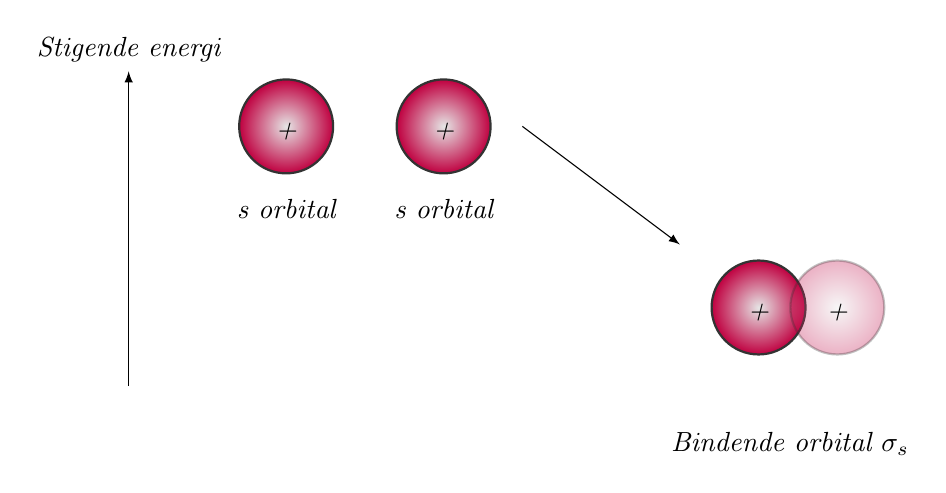
\begin{tikzpicture}[scale=2]
  \begin{scope}[font=\itshape]% 

  \draw[-latex] (0,-1)--(0,1) node[above]{Stigende energi};
  \orbital[color = purple, opacity = 1, scale = 2, pos = {(1,0.65)}]{s} 
  \orbital[color = purple, opacity = 1, scale = 2, pos = {(2,0.65)}]{s} 
  \node[above] at (1,0.5) {+};  
  \node[above] at (2,0.5) {+};
  \node[above] at (1,0) {s orbital};
  \node[above] at (2,0) {s orbital};
	\draw[-latex] (2.5,0.65)--(3.5,-0.10);
 		
 		
 		
 \orbital[color = purple, opacity = 1, scale = 2, pos = {(4,-0.5)}]{s} 
  \orbital[color = purple, opacity = 0.3, scale = 2, pos = {(4.5,-0.5)}]{s}  		
  \node[above] at (4.2,-1.5) {Bindende orbital $\sigma_s$};
 	\node[above] at (4,-0.65) {+}; 
 	\node[above] at (4.5,-0.65) {+}; 
  \end{scope}

  \begin{pgfonlayer}{backbackground}
  \fill[white](current bounding box.south west)rectangle
  (current bounding box.north east);
  \end{pgfonlayer}
  \end{tikzpicture}
  \caption{1s orbital} \end{figure}
	\end{center}
	
Denne bindende $\sigma$-orbital er faktisk det vi også kender som en $\sigma$-binding eller en kovalent binding. Kovalente bindinger er netop defineret som molekylære bindinger, der involverer at to atomer deler deres elektroner. 
\\

På samme måde som med $\sigma$-orbitalerne dannes $\pi$-orbitalerne ved, at to atomers befinder sig tæt på hinanden og elektronerne kan få en lavere energi ved at befinde sig i det sted hvor orbitalerne overlapper. $\pi$-orbitalerne adskiller sig alligevel fra $\sigma$-orbitalerne ved ikke at kunne blive dannet af overlap mellem s-orbitaler. En illustration af hvordan $\pi$-bindinger dannes ved et overlap af p-orbitaler: se figur 5. 

\begin{center}
\begin{figure}[ht!]
  \centering
  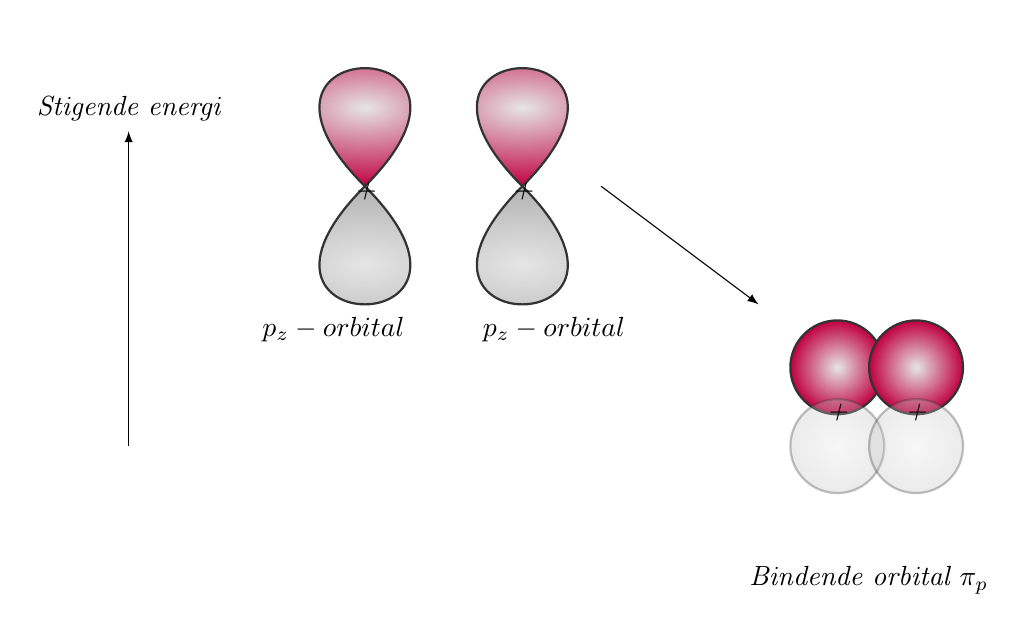
\begin{tikzpicture}[scale=2]
  \begin{scope}[font=\itshape]% 

  \draw[-latex] (-0.5,-1)--(-0.5,1) node[above]{Stigende energi};
  \orbital[pcolor = purple, opacity = 1, scale = 1, pos = {(1,0.65)}]{pz} 
  \orbital[pcolor = purple, opacity = 1, scale = 1, pos = {(2,0.65)}]{pz} 
  \node[above] at (0.8,-0.40) {$p_z-orbital$};
  \node[above] at (2.2,-0.40) {$p_z-orbital$};
	\draw[-latex] (2.5,0.65)--(3.5,-0.10);
  \node[above] at (1,0.5) {+};
  \node[above] at (2,0.5) {+};
 		
 \orbital[color = purple, opacity = 1, scale = 2, pos = {(4,-0.5)}]{s} 
  \orbital[color = purple, opacity = 1, scale = 2, pos = {(4.5,-0.5)}]{s}  	
  
 \orbital[color = lightgray, opacity = 0.3, scale = 2, pos = {(4,-1)}]{s} 
  \orbital[color = lightgray, opacity = 0.3, scale = 2, pos = {(4.5,-1)}]{s}  	  
  	
  \node[above] at (4.2,-2) {Bindende orbital $\pi_p$};
 		
 		
  \node[above] at (4,-0.90) {+};
  \node[above] at (4.5,-0.90) {+};		
 		
  \end{scope}

  \begin{pgfonlayer}{backbackground}
  \fill[white](current bounding box.south west)rectangle
  (current bounding box.north east);
  \end{pgfonlayer}
  \end{tikzpicture}
  \caption{1s orbital} \end{figure}
	\end{center}
\pagebreak
	
Nu har vi set på både $\sigma$-orbitaler /bindinger og $\pi$-orbitaler / bindinger - men hver for sig. Hvis de to orbitaler eksisterer sammentidigt i et molekyle har vi faktisk en dobbeltbinding. Dobbeltbindinger er netop en $\sigma$- og en $\pi$-binding. Illustret som en tegning ville det se ud på følgende måde, se Figur 6: 

\begin{center}
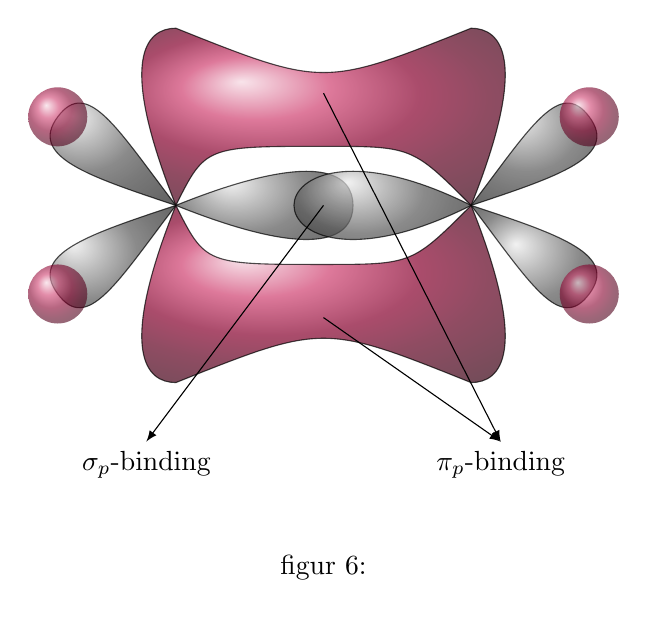
\begin{tikzpicture}[scale=0.75]

\shade[shading=ball, ball color=gray,draw,opacity=.7] (-2.5,0) .. controls (0,1) and     (.5,0.5) .. (.5,0)
.. controls (.5,-.5) and (0,-1) .. (-2.5,0);

\shade[shading=ball, ball color=gray,draw,opacity=.7] (2.5,0) .. controls (.5,1) and     (-.5,0.5) .. (-.5,0)
.. controls (-.5,-.5) and (.5,-1) .. (2.5,0);


\shade[shading=ball, ball color=gray,draw,opacity=.7] (-2.5,0) .. controls (-4,0.5) and     (-5,0.83) .. (-4.5,1.5)
.. controls (-4,2.17) and (-3.5,1.31) .. (-2.5,0);

\shade[shading=ball, ball color=gray,draw,opacity=.7] (-2.5,0) .. controls (-4,-0.5)     and (-5,-0.83) .. (-4.5,-1.5)
.. controls (-4,-2.17) and (-3.5,-1.31) .. (-2.5,0);


\shade[shading=ball, ball color=gray,draw,opacity=.7] (2.5,0) .. controls (4,0.5) and     (5,0.83) .. (4.5,1.5)
.. controls (4,2.17) and (3.5,1.31) .. (2.5,0);

\shade[shading=ball, ball color=gray,draw,opacity=.7] (2.5,0) .. controls (4,-0.5) and     (5,-0.83) .. (4.5,-1.5)
.. controls (4,-2.17) and (3.5,-1.31) .. (2.5,0);

\shade[shading=ball, ball color=purple,opacity=0.6] (4.5,1.5) circle (0.5);

\shade[shading=ball, ball color=purple,opacity=0.6] (4.5,-1.5) circle (.5);

\shade[shading=ball, ball color=purple,opacity=0.6] (-4.5,-1.5) circle (.5);

\shade[shading=ball, ball color=purple,opacity=0.6] (-4.5,1.5) circle (.5);


\shade[shading=ball, ball color=purple,draw,opacity=.7] (-2.5,0) .. controls (-3.5,2.5)     and (-3,3) .. (-2.5,3)
.. controls (0,2) .. (2.5,3)
.. controls (3,3) and (3.5,2.5) .. (2.5,0)
.. controls (1.5,1) .. (0,1)
.. controls (-2,1) .. (-2.5,0);


\shade[shading=ball, ball color=purple,draw,opacity=.7] (-2.5,0) .. controls (-3.5,-2.5)     and (-3,-3) .. (-2.5,-3)
.. controls (0,-2) .. (2.5,-3)
.. controls (3,-3) and (3.5,-2.5) .. (2.5,-0)
.. controls (1.5,-1) .. (0,-1)
.. controls (-2,-1) .. (-2.5,-0);

\draw[-latex] (0,0)--(-3,-4) node[below]{$\sigma_p$-binding};

\draw[-latex] (0,1.9)--(3,-4) node[below]{$\pi_p$-binding};

\draw[-latex] (0,-1.9)--(3,-4) node[below]{ };


\node[above] at (0,-6.5){figur 6: };
\end{tikzpicture}
\end{center}

$\sigma$-bindingerne er de stærkestee af de kovalente bindinger. Dernæst kommer $\pi$-bindingerne. blabla MO teori...


Det er nemmelig ikke alle atomer, der har mulighed for at danne kovalente bindinger imellem sig. Når 2 atomer går sammen om at danne en kovalent binding er det fordi, at de hver især er ustabile. At de er ustabile er ens betydende med, at de ikke har deres orbitaler af højeste energiniveau fyldt ud. Hver orbital vil gerne have en spin-op og en spin-ned elektron. Når nogle atomer så alligevel ikke vælger at gå sammen og danne en kovalent binding er det enten fordi, at de har for mange mange elektroner til, at de kun kan befinde sig mellem atomerne og danne en bindende $\sigma$-binding og derfor befinder sig i en orbital, der kræver et højere energiniveau og derfor er anti-bindende. 

\subsection{kovalente bindinger}
Så det vi fandt ud af i dette afsnit var, at når 2 atomer går sammen og deler deres elektroner for at opnå en lavere energitilstand dannes nogle bindinger som vi kalder kovalente bindinger. Kovalente bindinger dannes når atomer, der har lige stor tilbøjelighed til at afgive elektroner mødes. Et eksempel på et organisk molekyle, der dannes kovalente bindinger er ethylen. Her ses det tydeligt hvordan de to p-orbitaler går sammen i midten af molekylet om at lave en $\sigma_p$-(se figur 6). Delter elektroner findes primært mellem de positivt ladede atomkerner og den elektrostatiske tiltrækning mellem de to positivt ladede kerner og de to negativt ladede elektroner holder molekylet sammen. Det bånd der bliver dannet som et resultat af dette er meget stærkt. 



\end{document}